\documentclass[mathserif,handout]{beamer}
%\documentclass{beamer}
\usetheme{Warsaw}
\usecolortheme{seahorse}
\usecolortheme{orchid}
\usepackage{amsmath,verbatim}
\usepackage{listings}
\usepackage[english]{babel}
%\usepackage{movie15}
\setbeamercovered{transparent}

\newcommand{\Deltap}{\ensuremath{\Delta^{\!+}}}
\newcommand{\trans}{\ensuremath{{}^\mathrm{T}}}
\newcommand{\eps}{\varepsilon}
\newcommand*{\approxdist}{\mathrel{\vcenter{\offinterlineskip
\vskip-.25ex\hbox{\hskip.55ex$\cdot$}\vskip-.25ex\hbox{$\sim$}
\vskip-.5ex\hbox{\hskip.55ex$\cdot$}}}}

\lstdefinelanguage{myR}
{
   language=R,
   otherkeywords={read.table, set.seed, head},
   deletekeywords={url,codes, t, dt, Call, formula,Q, R, on,by,hat,is,
col, set,start,end,deltat,zip},
   sensitive=true,
   breaklines=true,
   morecomment=[l]{\#},
   morestring=[b]",
   morestring=[b]',
   basicstyle =\ttfamily\small,
   keywordstyle=\bfseries,
   showtabs=false,
   showstringspaces=false,
   literate= {~}{$\sim$}{2},
   numberstyle=\sffamily\scriptsize,
   stepnumber=2
 }


\begin{document}

\title[FP for scalable statistical computing]{Functional programming languages for scalable statistical computing}
\author[Darren Wilkinson --- Warwick, 27/2/15]{\textbf{\large Darren Wilkinson} \\
\alert{\url{http://tinyurl.com/darrenjw}}\\
School of Mathematics \& Statistics\\Newcastle University, UK}
\date{OxWaSP Symposium on Scalable methods,\\Warwick University,\\27th February 2015}

\frame{\titlepage}


\frame{
\frametitle{Outline}
\begin{itemize}
\item Parallelisation of Monte Carlo
\item MCMC (parallel chains and parallelised single chains)
\item Case study: SV Models
\item Scala, functional programming, immutable data structures and parallelisation
\item Summary
\end{itemize}
}


\section{Monte Carlo and Markov chain Monte Carlo}

\subsection{Monte Carlo}

\frame{
\frametitle{Monte Carlo}
\begin{itemize}
\item
\(
\displaystyle
\phi \sim \Pi \text{ and } \Pi \text{ has density } \pi(\phi)
\)
\item
\(
\displaystyle
I  = E_\Pi(t(\phi)) = \int t(\phi)d\Pi(\phi) = \int t(\phi)\pi(\phi)d\phi
\)
\item
\[
I \simeq \frac{1}{n} \sum_{i=1}^n t(\phi^{(i)})
\]
where $\phi^{(i)} \sim \Pi,\ i=1,2,\ldots n$.
\item
Very easy to parallelise! 
\item Suppose we have $N$ processors, where
$N|n$...
\end{itemize}
}

\frame{
\frametitle{Parallel Monte Carlo integral}
\begin{enumerate}
\item Master program computes $m=n/N$, and passes $m$ to each 
	available processor
\item Each processor ($k$):
	\begin{enumerate}
	\item simulates $m$ independent realisations of $\phi$
	\item computes $S_k = \sum_{i=1}^m t(\phi^{(i)})$
	\item passes $S_k$ back to master program
	\end{enumerate}
\item Master program collects and sums the $S_k$ to give final sum
$S$.
\item Master program returns $S/n$
\end{enumerate}
Need to be careful about independence of random numbers across
processors --- need to understand how PRNG works...
}

\begin{comment}

\subsection{Parallel pseudo-random number generation}

\frame{
\frametitle{PRNG: pseudo-random number generation}

How does it work?

\setlength{\unitlength}{0.8cm}
\begin{picture}(12,5)
\put(0,2.5){$S_0$}
\put(2,2.5){$S_1$}
\put(4,2.5){$S_2$}
\put(10,2.5){$S_{i-1}$}
\put(12,2.5){$S_i$}
\multiput(0.6,2.68)(2,0){6}{\vector(1,0){1.3}}
\multiput(1.1,2.9)(2,0){6}{$\psi$}
\multiput(2.2,2.3)(2,0){6}{\vector(0,-1){1.3}}
\multiput(2.3,1.7)(2,0){6}{$\rho$}
\put(2,0.5){$u_1$}
\put(4,0.5){$u_2$}
\put(10,0.5){$u_{i-1}$}
\put(12,0.5){$u_i$}
\put(0.1,4.5){$s$}
\put(0.2,4.4){\vector(0,-1){1.5}}
\put(0.3,3.6){$\omega$}
\end{picture}

Actually a big loop (circle), as the state has finite size, and
therefore must eventually return to the original state and cycle.
}


\frame{
\frametitle{PPRNG: parallel pseudo-random number generation}
Problems with multiple processors:
\begin{itemize}
\item Can't share a single stream (too much overhead)
\item Can't use identical streams
\item ``Different seeds'' doesn't completely solve the problem
	\begin{itemize}
	\item this just starts you on a different part of the state
``loop'' --- danger of overlapping streams if seeding is not
sophisticated or simulation is large
	\end{itemize}	
\item Need independent streams on each processor...
	\begin{itemize}
	\item ie. want states to lie on a toroidal lattice rather than
a circular lattice
	\end{itemize}
\end{itemize}
}

\frame{
\frametitle{PPRNG mappings}
\setlength{\unitlength}{0.6cm}
\begin{center}
\begin{picture}(12,12)
\newsavebox{\onestream}
\savebox{\onestream}(12,3.5)[bl]{
\put(0,2.5){$S_0$}
\put(2,2.5){$S_1$}
\put(4,2.5){$S_2$}
\put(10,2.5){$S_{i-1}$}
\put(12,2.5){$S_i$}
\multiput(0.6,2.68)(2,0){6}{\vector(1,0){1.3}}
\multiput(1.1,2.9)(2,0){6}{$\psi$}
\multiput(2.2,2.3)(2,0){6}{\vector(0,-1){1.3}}
\multiput(2.3,1.7)(2,0){6}{$\rho$}
\put(2,0.5){$u_1$}
\put(4,0.5){$u_2$}
\put(10,0.5){$u_{i-1}$}
\put(12,0.5){$u_i$}
}
\put(1,0){\usebox{\onestream}}
\put(1,4){\usebox{\onestream}}
\put(1,8){\usebox{\onestream}}
\multiput(1.3,2.8)(2,0){3}{\scriptsize$3$}
\multiput(11.3,2.8)(2,0){2}{\scriptsize$3$}
\multiput(1.3,6.8)(2,0){3}{\scriptsize$2$}
\multiput(11.3,6.8)(2,0){2}{\scriptsize$2$}
\multiput(1.3,10.8)(2,0){3}{\scriptsize$1$}
\multiput(11.3,10.8)(2,0){2}{\scriptsize$1$}
\multiput(3.25,0.7)(2,0){2}{\scriptsize$3$}
\multiput(11.25,0.7)(2,0){2}{\scriptsize$3$}
\multiput(3.25,4.7)(2,0){2}{\scriptsize$2$}
\multiput(11.25,4.7)(2,0){2}{\scriptsize$2$}
\multiput(3.25,8.7)(2,0){2}{\scriptsize$1$}
\multiput(11.25,8.7)(2,0){2}{\scriptsize$1$}
\put(-1,6.5){$s$}
\put(-0.6,6.7){\vector(1,0){1.5}}
\put(-0.7,7.0){\vector(1,2){1.6}}
\put(-0.7,6.4){\vector(1,-2){1.6}}
\put(0,6.8){$\omega^2$}
\put(-0.3,8.8){$\omega^1$}
\put(-0.5,4.8){$\omega^3$}
\end{picture}
\end{center}
}


\frame{
\frametitle{Example Monte Carlo Integral}

Consider numerical evaluation of the integral
\[
I = \int_0^1 \exp\{-u^2\} du = E_U(\exp\{-U^2\}) \simeq \frac{1}{n}
\sum_{i=1}^n \exp\{-u_i^2\}
\]
where
\[
u_i \sim U(0,1).
\]
}

%\frame{
\begin{frame}[fragile]
\frametitle{Parallel Monte Carlo integral (C+MPI+SPRNG)}
% monte-carlo.c
{\scriptsize
\begin{lstlisting}[language=C]
int main(int argc,char *argv[])
{
  int i,k,N; double u,ksum,Nsum; gsl_rng *r;
  MPI_Init(&argc,&argv);
  MPI_Comm_size(MPI_COMM_WORLD,&N);
  MPI_Comm_rank(MPI_COMM_WORLD,&k);
  r=gsl_rng_alloc(gsl_rng_sprng20);
  for (i=0;i<10000;i++) {
    u = gsl_rng_uniform(r);
    ksum += exp(-u*u);
  }
  MPI_Reduce(&ksum,&Nsum,1,MPI_DOUBLE,MPI_SUM,0,MPI_COMM_WORLD);
  if (k == 0) {
    printf("Monte carlo estimate is %f\n", (Nsum/10000)/N );
  }
  MPI_Finalize();
  exit(EXIT_SUCCESS);
}
\end{lstlisting}
}
\end{frame}
%}

\end{comment}

\subsection{Parallel MCMC}

\frame{
\frametitle{MCMC: Parallel chains}

Multiple parallel chains is really easy...
\vspace*{0.8ex}

\textbf{\large Example}

\begin{itemize}
\item Metropolis-Hastings for a standard normal random quantity based on
$U(-\alpha,\alpha)$ innovations.
\item So if chain is currently at $x$, a new candidate $x^\star$ is
simulated from $U(x-\alpha,x+\alpha)$, and this candidate is accepted
with probability $\min\{1,A\}$, where
\[
A  = \phi(x^\star) / \phi(x)
\]
and $\phi(\cdot)$ is the standard normal density.
\end{itemize}
}

%\frame{
\begin{frame}[fragile]
\frametitle{Independent parallel MCMC chains}
% mcmc.c
{\scriptsize
\begin{lstlisting}[language=C]
#include <gsl/gsl_rng.h>
#include "gsl-sprng.h"
#include <gsl/gsl_randist.h>
#include <mpi.h>

int main(int argc,char *argv[])
{
  int k,i,iters; double x,can,a,alpha; gsl_rng *r;
  FILE *s; char filename[15];
  MPI_Init(&argc,&argv);
  MPI_Comm_rank(MPI_COMM_WORLD,&k);
  if ((argc != 3)) {
    if (k == 0)
      fprintf(stderr,"Usage: %s <iters> <alpha>\n",argv[0]);
    MPI_Finalize(); return(EXIT_FAILURE);
  }
  iters=atoi(argv[1]); alpha=atof(argv[2]);
  r=gsl_rng_alloc(gsl_rng_sprng20);
\end{lstlisting}
}
\end{frame}

\begin{frame}[fragile]
\frametitle{ctd.}
{\scriptsize
\begin{lstlisting}[language=C]
  sprintf(filename,"chain-%03d.tab",k);
  s=fopen(filename,"w");
  if (s==NULL) {
    perror("Failed open");
    MPI_Finalize(); return(EXIT_FAILURE);
  }
  x = gsl_ran_flat(r,-20,20);
  fprintf(s,"Iter X\n");
  for (i=0;i<iters;i++) {
    can = x + gsl_ran_flat(r,-alpha,alpha);
    a = gsl_ran_ugaussian_pdf(can) / gsl_ran_ugaussian_pdf(x);
    if (gsl_rng_uniform(r) < a)
      x = can;
    fprintf(s,"%d %f\n",i,x);
  }
  fclose(s);
  MPI_Finalize(); return(EXIT_SUCCESS);
}
\end{lstlisting}
}
\end{frame}
%}

\frame{
\frametitle{Parallel chains MCMC}
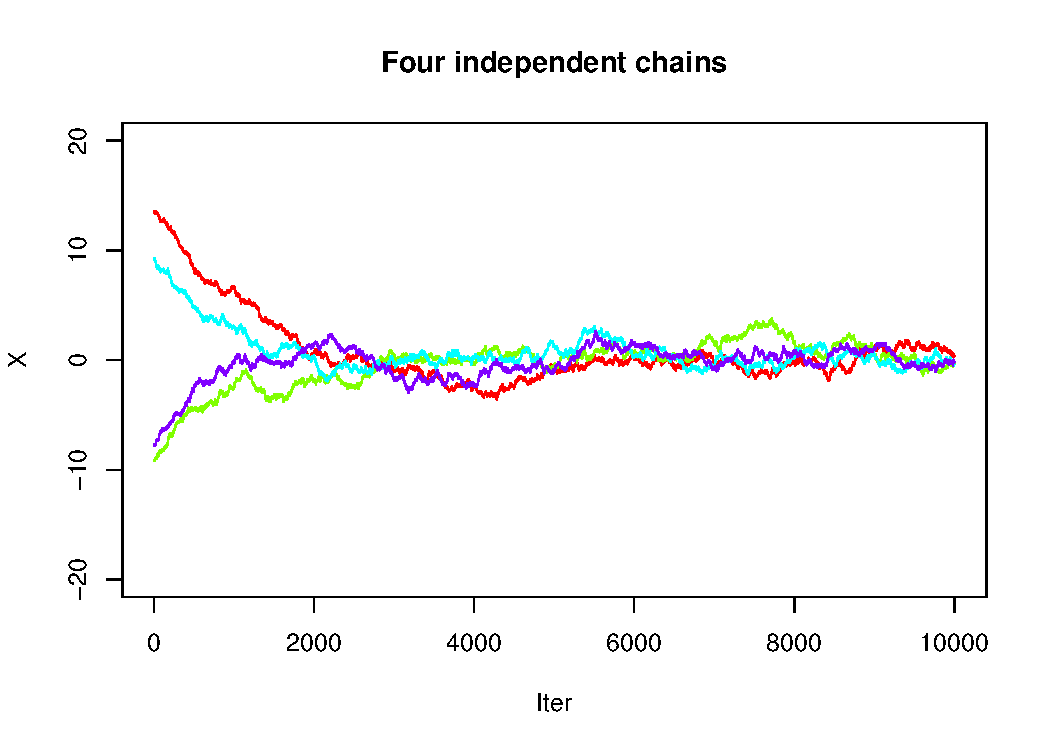
\includegraphics[width=\textwidth]{mcmc-trace}
}

\frame{
\frametitle{Burn-in and speed-up with parallel chains}

\begin{itemize}
\item
If burn-in is $b$ and $n$ iterations are required for the monitoring
run, then
\end{itemize}
\begin{block}{Speed-up}
\[
SpeedUp(N) = \frac{b+n}{b+\frac{n}{N}} \longrightarrow \frac{b+n}{b}
\]
\end{block}
\begin{itemize}
\item
So speed-up is bounded as the number of processors tends to infinity!
\item This is essentially \alert{Amdahl's law} for parallel chains
MCMC...
\end{itemize}
}

\frame{
\frametitle{Parallel chains speed-up for $n=10b$}
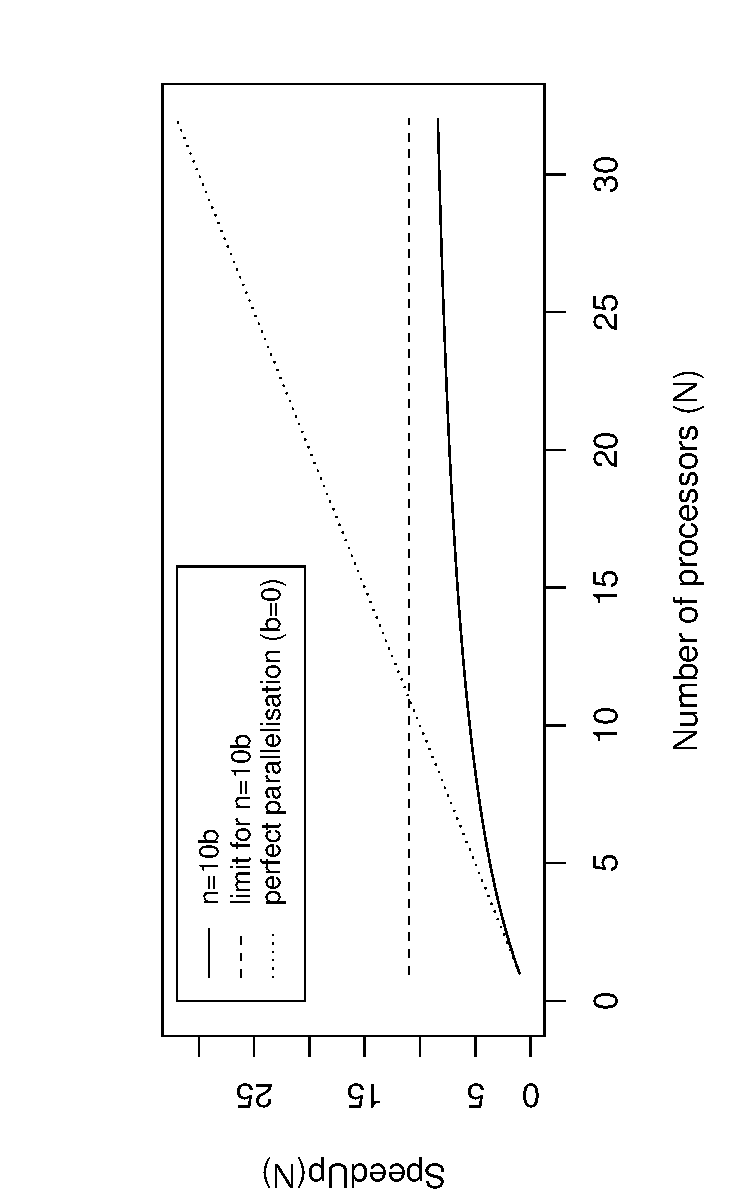
\includegraphics[width=0.6\textwidth,angle=270]{speedup}
}

\frame{
\frametitle{Parallelising single chains}
\begin{itemize}
\item The problem with parallelising MCMC chains is that each proposed
new state depends on the previous state, essentially making it
difficult to farm out multiple iterations to different processors
\item A couple of exceptions:
	\begin{itemize}
	\item For a Metropolis \alert{independence}
	sampler where the evaluation of the likelihood of the proposal
	is time consuming, it is possible to generate many candidates
	and evaluate likelihoods on multiple processors
	\item
	\alert{pre-fetching}: given a (single-block, or random sweep) M-H
	algorithm, can farm out all $2^n$ likelihood evaluations which
	might be required in order to advance the chain by $n$ steps
	(but speed-up is only logarithmic in number of processors)
	\end{itemize}
\item Otherwise need to parallelise each iteration...
\end{itemize}
}

\frame{
\frametitle{Parallelised single chain}
Exploit conditional independence...
\begin{itemize}
\item
\(
\pi(\sigma,\theta,y) = \pi(\sigma)\pi(\theta|\sigma)p(y|\sigma,\theta)
\)
\item
\(
\sigma=(\sigma_1,\ldots,\sigma_p),\quad \theta=(\theta_1,\ldots,\theta_q)
\)
\item
Update of $\sigma$ is fast. 
\item Update of $\theta$ is slow. 
\item Parallelise
update of $\theta$.
\item
Simplest case: $\theta_i \perp\hspace{-0.8ex}\perp \theta_j |\sigma,y$
\end{itemize}
}

\frame{
\frametitle{Basic algorithm}
\begin{enumerate}
\item Each processor ($k$):
	\begin{enumerate}
	\item sequentially updates the $q_k$ $\theta$s that have been
assigned to it, using the current value of $\sigma$
	\item computes summary statistics for the new $\theta$s that
will be required to update $\sigma$
	\item passes the summary statistics back to the root process
(master program)
	\end{enumerate}
\item The root process combines the summary statistics in order to
obtain an explicit form for the updating of $\sigma$
\item A new $\sigma$ is sampled and output
\item The new $\sigma$ is distributed out to each process
\end{enumerate}
}

\frame{
\frametitle{Serial dependence}

\begin{block}{Markov dependence}
\[
\theta_i \perp\hspace{-0.8ex}\perp
\theta_j|\theta_{i-1},\theta_{i+1},\sigma,y,\quad j\not= i
\]
\end{block}
\setlength{\unitlength}{0.8cm}
\begin{picture}(13,2)
\multiput(1,1)(2,0){6}{\circle{1}}
\multiput(1.5,1)(2,0){6}{\line(1,0){1}}
\put(0.9,0.9){$\theta_1$}
\put(2.9,0.9){$\theta_2$}
\put(4.9,0.9){$\theta_3$}
\put(6.9,0.9){$\theta_4$}
\put(8.9,0.9){$\theta_5$}
\put(10.9,0.9){$\theta_6$}
\end{picture}
\begin{itemize}
\item
Note that the ``odd'' numbered blocks are conditionally independent of
one another given the ``even'' numbered blocks, and vice versa.
\end{itemize}
}

\frame{
\frametitle{MRF example}
\setlength{\unitlength}{0.8cm}
\begin{picture}(13,9)
\multiput(1,1)(2,0){6}{\circle{1}}
\multiput(1.5,1)(2,0){6}{\line(1,0){1}}
\multiput(1,1.5)(2,0){6}{\line(0,1){1}}
\multiput(1,3)(2,0){6}{\circle{1}}
\multiput(1.5,3)(2,0){6}{\line(1,0){1}}
\multiput(1,3.5)(2,0){6}{\line(0,1){1}}
\multiput(1,5)(2,0){6}{\circle{1}}
\multiput(1.5,5)(2,0){6}{\line(1,0){1}}
\multiput(1,5.5)(2,0){6}{\line(0,1){1}}
\multiput(1,7)(2,0){6}{\circle{1}}
\multiput(1.5,7)(2,0){6}{\line(1,0){1}}
\multiput(1,7.5)(2,0){6}{\line(0,1){1}}
\multiput(1,1)(4,0){3}{\circle*{0.3}}
\multiput(3,3)(4,0){3}{\circle*{0.3}}
\multiput(1,5)(4,0){3}{\circle*{0.3}}
\multiput(3,7)(4,0){3}{\circle*{0.3}}
\end{picture}
}

\frame{
\frametitle{General dependence structures}
\begin{itemize}
\item
Need to divide up the blocks of $\theta$ into sets of blocks which are
conditionally independent, and hence can be updated in parallel.
\item
$T=\{T_1,\ldots,T_c\}$ is a \alert{partition} of
$\{\theta_1,\ldots,\theta_q\}$ where each $T_i$ is a set of blocks
that are conditionally independent given all remaining blocks (and
$\sigma$ and $y$). 
\item
The smallest $c$ for which this is possible is known as the
\alert{chromatic} number of the graph. Finding this number and a
suitable partition is the \alert{graph colouring problem} --- NP hard
in general.
\end{itemize}
}

\frame{
\frametitle{General algorithm}

\begin{enumerate}
\item Each processor ($k$):
	\begin{enumerate}
	\item For each $i$ in 1 to $c$:
		\begin{enumerate}
		\item sequentially updates all the blocks in $T_i$ 
			allocated to it
		\item distributes necessary state information
regarding updates to adjacent processors
		\item receives such information from adjacent processors
		\end{enumerate}
	\item computes summary statistics for the new $\theta$s that
will be required to update $\sigma$
	\item passes the summary statistics back to the root process
(master program)
	\end{enumerate}
\item the root process combines the summary statistics in order to
obtain an explicit form for the updating of $\sigma$
\item a new $\sigma$ is sampled and output
\item the new $\sigma$ is distributed out to each process
\end{enumerate}
}

\begin{comment}

\frame{
\frametitle{When elements of $\sigma$ are not CI:}

\begin{enumerate}
\item Each processor ($k$):
	\begin{enumerate}
	\item for each $i$ in 1 to $c$:
		\begin{enumerate}
		\item sequentially updates all the blocks in $T_i$ 
			allocated to it
		\item distributes necessary state information
regarding updates to adjacent processors
		\item receives such information from adjacent processors
		\end{enumerate}
	\end{enumerate}
\item for each $i$ in 1 to $p$:
	\begin{enumerate}
	\item each processor (k):
		\begin{enumerate}
		\item computes summary statistics that
will be required to update $\sigma_i$
		\item passes the summary statistics back to the root process
		\end{enumerate}
	\item the root process combines the summary statistics in order to
obtain an explicit form for the updating of $\sigma_i$
	\item a new $\sigma_i$ is sampled and output
	\item the new $\sigma_i$ is distributed out to each processor
	\end{enumerate}
\end{enumerate}
}

\end{comment}

\subsection{Case study}

\frame{
\frametitle{Case study: SV models}

\begin{block}{Stochastic volatility model}
\begin{align*}
y_t &= \varepsilon_t\exp\{\alpha_t/2\}, \\
\alpha_t &= \mu + \phi(\alpha_t-\mu) + \eta_t,\quad t=1,2,\ldots,n \\
\varepsilon_t &\sim N(0,1),\quad \eta_t \sim N(0,\sigma_\eta^2)
\end{align*}
\end{block}
\begin{itemize}
\item
Can re-write first equation as
\[
\log y_t^2 = \alpha_t + \log(\varepsilon_t^2)
\]
\item
Use approximation $\log(\varepsilon_t^2) \sim N(-1.27,\pi^2/2)$ to get
a DLM.
\item
Basic idea: divide $\alpha$s up into blocks. Propose update for each
block using a sample from approximating DLM. Correct approximation
using a Metropolis-Hastings step. 
\end{itemize}
}

\frame{
\frametitle{Parallel updating scheme}

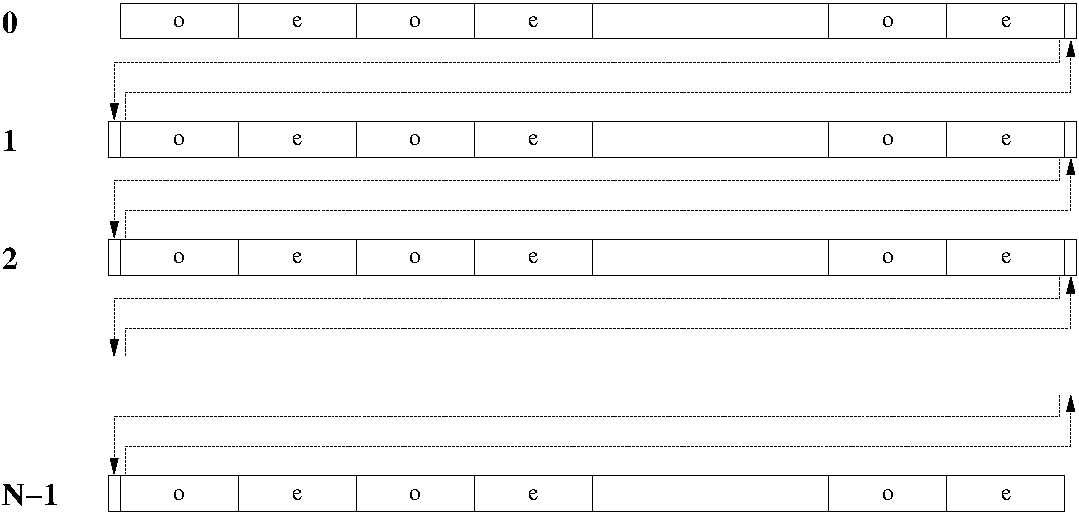
\includegraphics[width=\textwidth]{message}
}

\frame{
\frametitle{MCMC output}
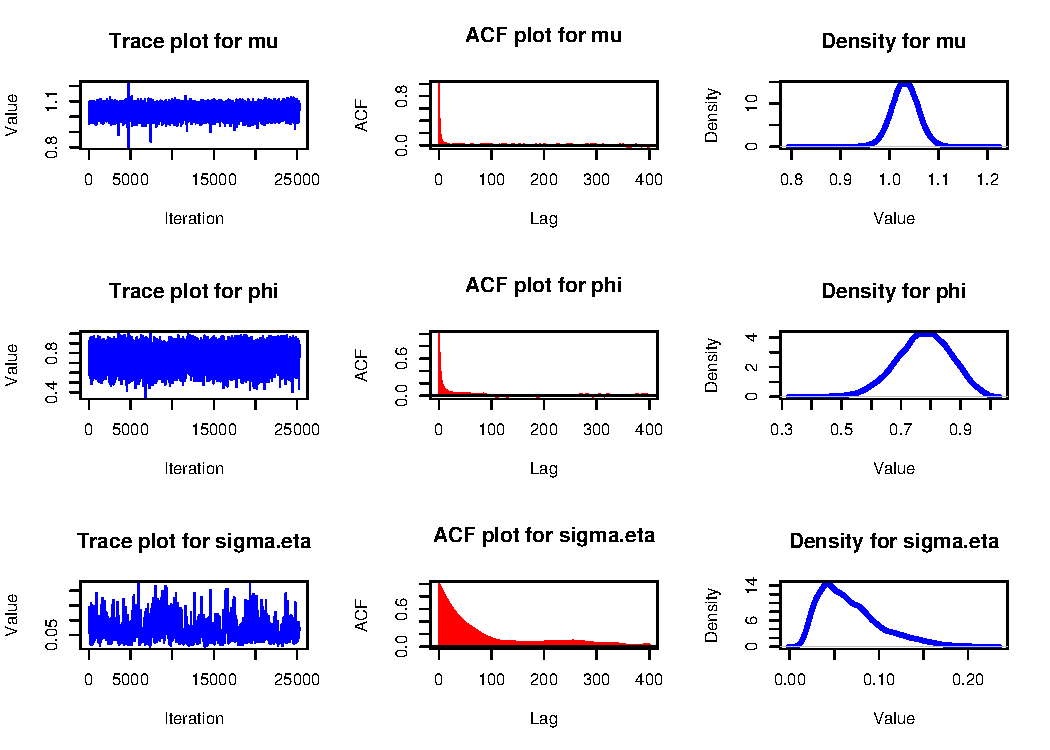
\includegraphics[width=0.9\textwidth]{case-trace}
}

\frame{
\frametitle{Empirical performance}
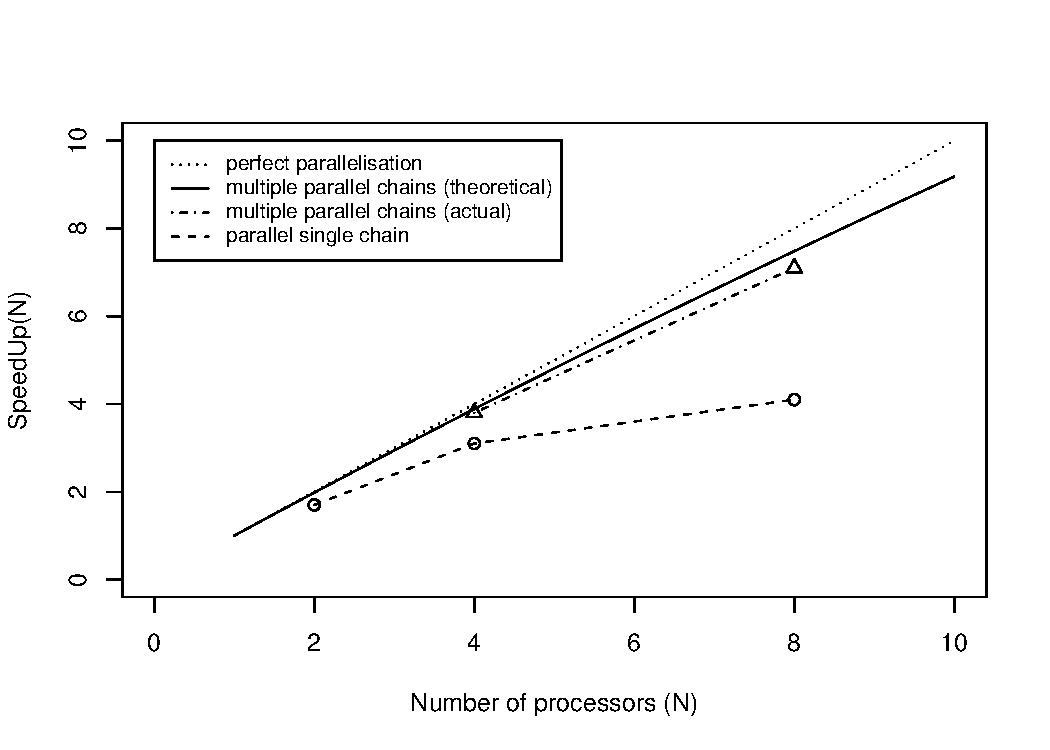
\includegraphics[width=0.9\textwidth]{case-speed}
}

\begin{comment}

\section{Likelihood free Monte Carlo algorithms}

\subsection{ABC}


\frame{
\frametitle{Alternative: approximate Bayesian computation (ABC)}
\begin{itemize}
\item Since
  $\pi(\theta,\mathbf{x},\mathcal{Y})=\pi(\theta)\pi(\mathbf{x}|\theta)\pi(\mathcal{Y}|\theta,\mathbf{x})$, it is trivial to generate samples from $\pi(\theta,\mathbf{x},\mathcal{Y})$ and to marginalise these down to $\pi(\theta,\mathcal{Y})$ 
\item Exact rejection algorithm: generate
  $(\theta^\star,\mathcal{Y}^\star)$ from $\pi(\theta,\mathcal{Y})$
  and keep provided that $\mathcal{Y}=\mathcal{Y}^\star$ otherwise
  reject and try again
\item This gives exact realisations from $\pi(\theta|\mathcal{Y})$,
  but in practice the acceptance rate will be very small (or zero)
\item ABC: Define a metric on the sample space, $\rho(\cdot,\cdot)$,
  and accept $(\theta^\star,\mathcal{Y}^\star)$ if
  $\rho(\mathcal{Y},\mathcal{Y}^\star)<\eps$
\item  This gives exact realisations from
  $\pi(\theta|\rho(\mathcal{Y},\mathcal{Y}^\star)<\eps)$, which tends
  to the true posterior as $\eps\longrightarrow 0$
\item Still problematic if there is a large discrepancy between the
  prior and posterior...
\end{itemize}
}

\frame{
\frametitle{ABC--SMC}
\begin{itemize}
\item Interest in a Bayesian posterior distribution
\[
\pi(\theta|x) \propto \pi(\theta)f(x|\theta)
\]
where $f(x|\theta)$ is intractable
\item Observed data $x_0$
\item Sequence of approximations
\[
\pi_t(\theta) = \pi(\theta|\rho(x,x_0)<\eps_t),
\]
where $\infty=\eps_0>\eps_1>\cdots>\eps_n>0$ and $\rho(\cdot,\cdot)$
is a suitable metric on data space
\item $\pi_0$ is the prior, and for sufficiently small $\eps_n$,
  hopefully $\pi_n$ not too far from the posterior, $\pi(\theta|x_0)$
\item Progressively reduce tolerances to improve agreement between
  successive distributions and hopefully improve acceptance rates
\end{itemize}
}

\frame{
\frametitle{ABC--SMC algorithm}
\begin{itemize}
\item Suppose we have a large (possibly weighted) sample of size $N$
  from $\pi_{t-1}(\theta)$, $\{\theta_1,\ldots,\theta_N\}$ with
  normalised weights $\tilde{w}_{t-1}^i$
\item Pick $\theta_i^\star \sim \pi_{t-1}(\theta)$ (weighted
  particles)
\item Perturb $\theta_i^{\star\star}\sim
  K(\theta_i^\star,\theta_i^{\star\star})$
\item Simulate $x^\star\sim f(x^\star|\theta^{\star\star})$ from
  intractable likelihood model
\item Accept only if $\rho(x^\star,x_0)<\eps_t$, otherwise reject go back to
  the start and pick another $\theta_i^\star$
\item Keep $\theta^{\star\star}$ as $i$th member of new sample, and
  compute its weight as
\[
w_t^i = \frac{\pi(\theta^{\star\star})}{\sum_{j=1}^N
  \tilde{w}_{t-1}^i K(\theta_j,\theta^{\star\star})}
\]
\item Once a sample of size $N$ is obtained, normalise weights and
  increment $t$
\end{itemize}
Parallelises well, but is approximate.
}

\subsection{pMCMC}

\frame{
\frametitle{Particle marginal Metropolis--Hastings (PMMH)}
\begin{itemize}
\item Use a particle filter to simulate an approximate sample from
  $\pi(\mathbf{x}|\mathcal{Y},\theta)$
\item Correct the acceptance probability to ensure that the target of
  the MCMC scheme is still the exact posterior
  $\pi(\theta,\mathbf{x}|\mathcal{Y})$
\item If a bootstrap particle filter is used, then this relies only on
  the ability to forward simulate from the process, and the entire
  procedure is ``likelihood--free''
\item pMCMC is the only obvious practical option for constructing
  global likelihood--free MCMC algorithms which are exact
  (\alert{Andrieu et al., 2010})
\item See \alert{Golightly \& W (2011)} for applications to POMP models
\end{itemize}
}

\frame{
\frametitle{``Sticking'' and tuning of PMMH}
\begin{itemize}
\item As well as tuning the $\theta$ proposal variance, it is
  necessary to tune the number of particles, $N$ in the particle filter ---
  need enough to prevent the chain from sticking, but computational
  cost roughly linear in $N$
\item
Number of particles necessary depends on $\theta$, but don't know
$\theta$ \emph{a priori}
\item Initialising the sampler is non-trivial, since much of parameter
  space is likely to lead to likelihood estimates that are numerically
  equal to zero --- how to move around when both current and proposed
  values have zero likelihood?!
\item Without careful tuning and initialisation, burn-in, convergence
  and mixing can all be very problematic...
\end{itemize}
}

\frame{
\frametitle{Adaptive ABC--SMC}
\begin{itemize}
\item PMMH algorithms require careful tuning, and are not trivial to
  parallelise 
\item Multiple parallel chains benefit from being initialised at
  samples from the posterior, in order to minimise burn-in
\item Tuning the number of particles to use in the particle filter is
  best done by averaging over a sample from the posterior
\item Adaptive ABC--SMC can be used to generate a sample from an
  approximation to the posterior, which is good enough for tuning and
  initialisation of PMMH chains
  \begin{itemize}
  \item ABC algorithms parallelise well, so this strategy is well
    suited to taking advantage of parallel hardware
  \item ABC--SMC algorithms also require tuning, but reasonable
    default choices work mostly OK for POMP models
  \end{itemize}
\item Multiple independent tuned PMMH chains can then target the exact
  posterior
\end{itemize}
}

\frame{
\frametitle{Comparing adaptive ABC--SMC against pMCMC}
\centerline{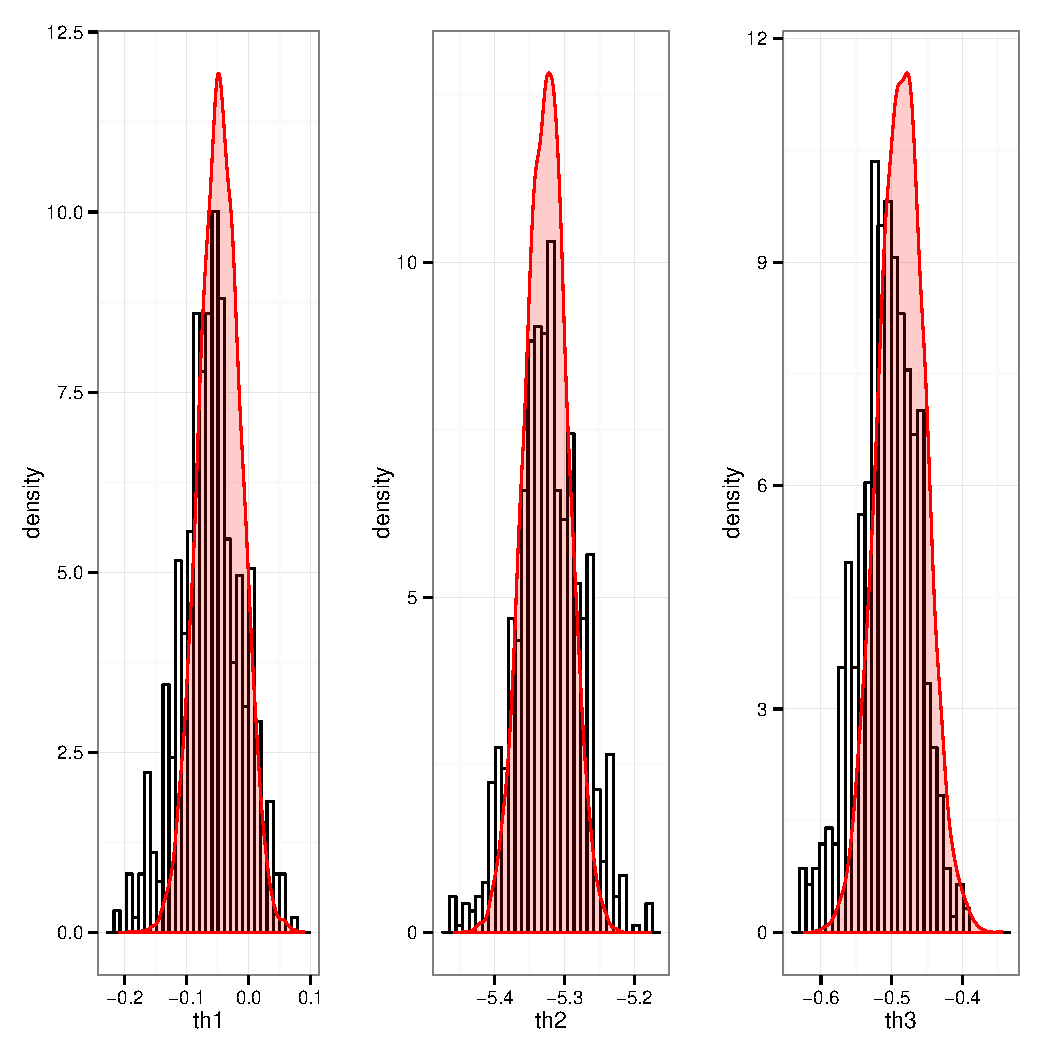
\includegraphics[width=0.6\textwidth]{abcplot}}

Observations on both species with known noise
}

\frame{
\frametitle{PMMH chains}

\centerline{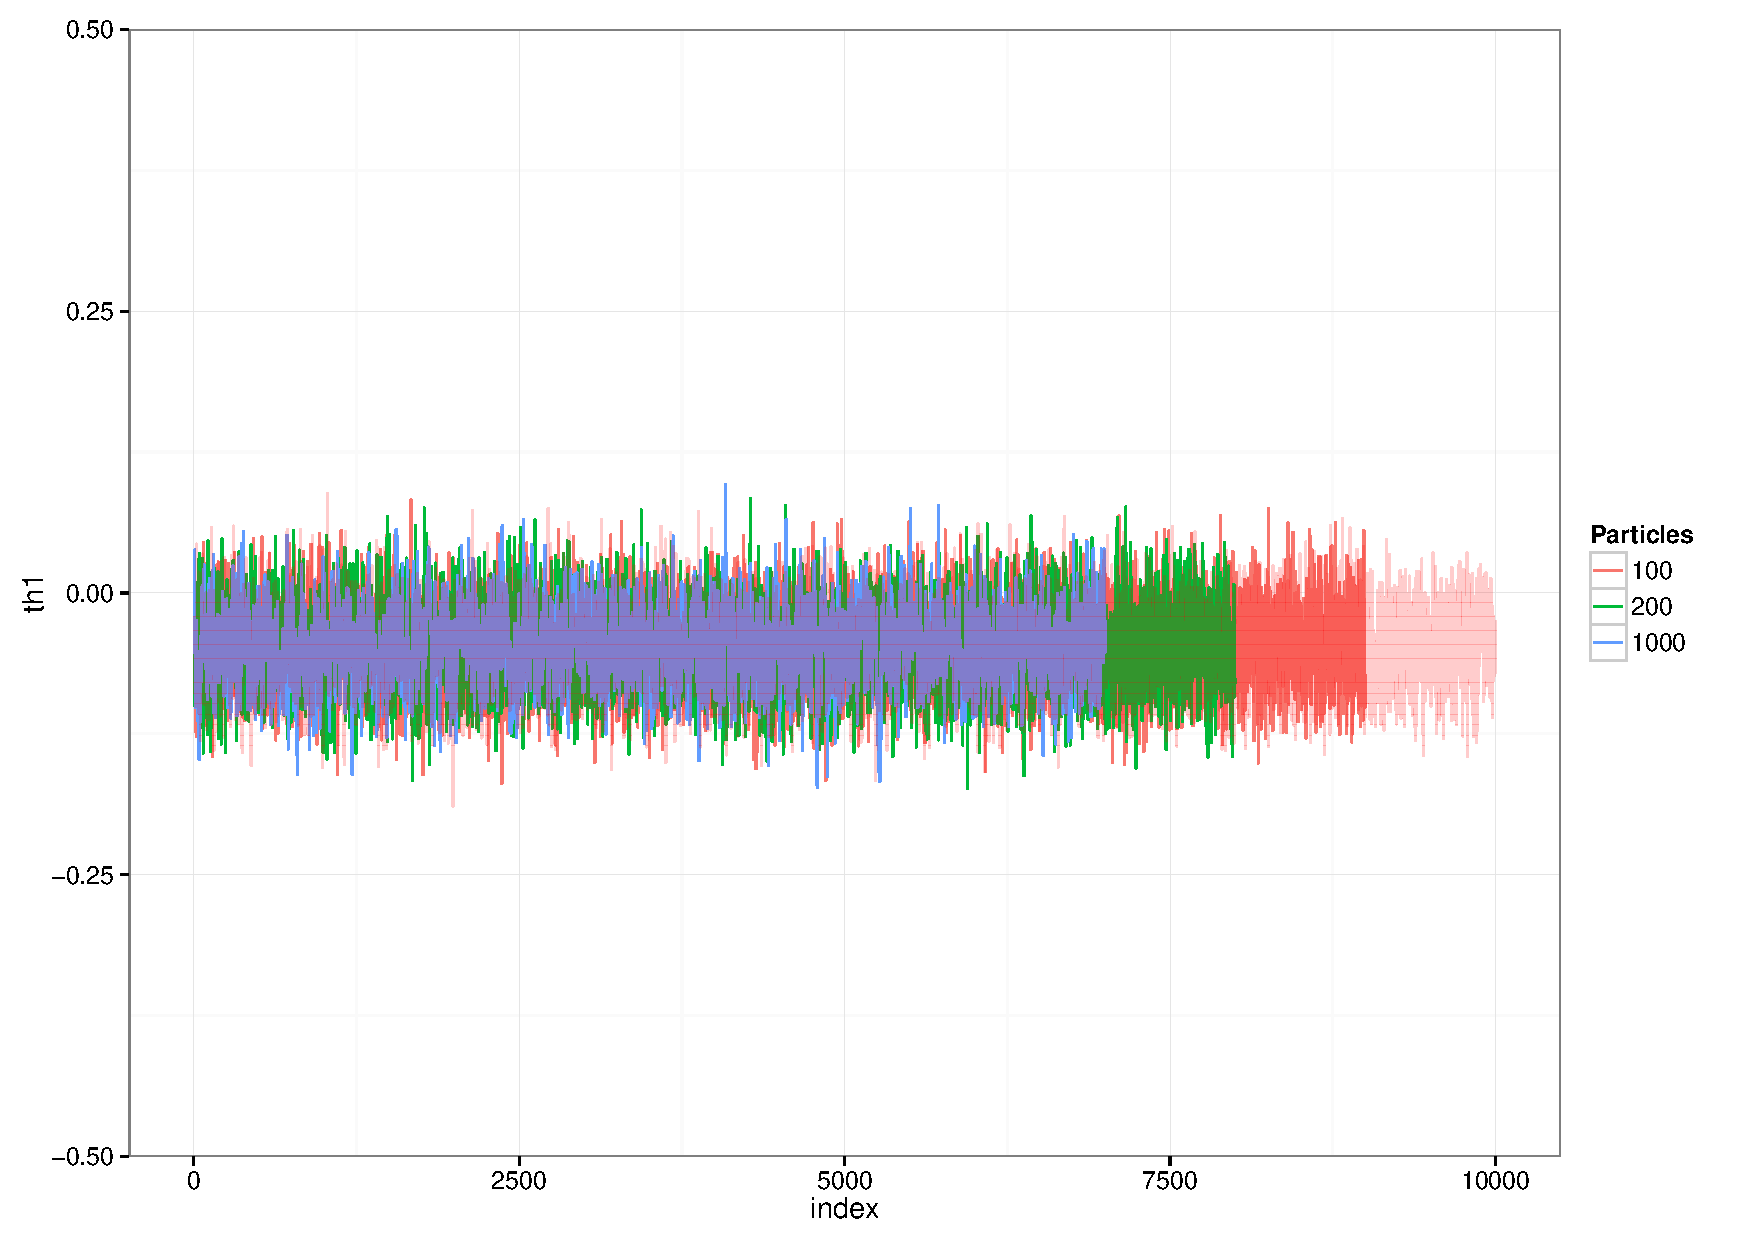
\includegraphics[width=0.8\textwidth]{pmcmcConverganceusingabc}}

PMMH chains initialised using samples from the ABC--SMC posterior (joint work with Jamie Owen and Colin Gillespie)
}

\subsection{SMC}

\frame{
\frametitle{SMC}
\begin{itemize}
\item What's up with parallelising SMC?!
\item I claimed that ABC--SMC parallelises well and that pMCMC doesn't
\item But they both have SMC in the inner loop --- how can that be?!
\item Granularity!
\item In ABC--SMC there will only be a handful of normalisation and resampling steps in total
\item In pMCMC there may be $T$ resampling steps per iteration, and there could be millions of iterations...
\end{itemize}
}

\begin{frame}[fragile]
\frametitle{Parallel particle filter in R}
{\small
\begin{lstlisting}[language=myR]
function(...) {
    xmat = simx0(n, t0, ...)
    ll = 0
    for (i in 1:length(deltas)) {
    xmat=t(sapply(mclapply(split(xmat,row(xmat)), stepFun, t0=times[i], deltat=deltas[i], ...),cbind))
        w = apply(xmat, 1, dataLik, t = times[i + 1], y = data[i,], log = FALSE, ...)
        ll = ll + log(mean(w))
        rows = sample(1:n, n, replace = TRUE, prob = w)
        xmat = xmat[rows, ]
    }
    ll
}
\end{lstlisting}
}
\end{frame}

\section{Functional programming}

\subsection{Functional approach to parallelism}

\frame{
\frametitle{Functional approaches to concurrency and parallelisation}
\begin{itemize}
\item Previous code written a rather functional style --- a function returning a function closure that uses ``map" and ``reduce" operations
\item Not lots of nested ``for" loops and imperative directives working with \alert{shared mutable state} (difficult for concurrency --- locks and synchronisation issues)
\item Functional languages, \alert{immutable state}, and \alert{referentially transparent} (\alert{side-effect} free) declarative workflow patterns are widely used for systems which really need to scale (leads to naturally parallel code)
\item Different sorts of ``scale" including:
  \begin{itemize}
  \item Scaling to big computations for relatively small data (HPC)
  \item Scaling to big models and/or data --- more like distributed computing
  \end{itemize}
\end{itemize}
}

\begin{frame}[fragile]
\frametitle{Parallel Monte Carlo integral in Scala}
{\scriptsize
\begin{lstlisting}[language=java]
object MonteCarlo {
  @tailrec
  def sum(its: Long,acc: Double): Double = {
    if (its==0) 
      (acc)
    else {
      val u=ThreadLocalRandom.current().nextDouble()
      sum(its-1,acc+exp(-u*u))
    }
  }
  def main(args: Array[String]) = {
    val N=args(0).toInt
    val iters=1000000000
    val its=iters/N
    val sums=(1 to N).toList.par map {x => sum(its,0.0)}
    val result=sums.reduce(_+_)
    println(result/iters)
  }
}
\end{lstlisting}
}
Actually runs \alert{faster} than the C+MPI version...
\end{frame}

\subsection{Functors, applicatives, monoids, monads, ...}

\frame{
\frametitle{Category theory}
Dummies guide:
\begin{itemize}
\item A ``collection" (or parametrised ``container" type) together with a ``map" function (defined in a sensible way) represents a \alert{functor}
\item If the collection additionally supports a (sensible) ``apply" operation, it is an \alert{applicative}
\item If the collection additionally supports a (sensible) ``flattening" operation, it is a \alert{monad} (required for composition)
\item For a ``reduce" operation on a collection to parallellise cleanly, the type of the collection together with the reduction operation must define a \alert{monoid} (must be an \alert{associative} operation, so that reductions can proceed in multiple threads in parallel)
\end{itemize}

}

\frame{
\frametitle{Monoids}
\centerline{$x_1+x_2+x_3+x_4=((x_1+x_2)+x_3)+x_4=(x_1+x_2)+(x_3+x_4)$}
\vspace{1ex}

Some examples from this workshop:
\begin{itemize}
\item Summing up (averaging) Monte Carlo samples to estimate an expectation
\item Pooling Monte Carlo samples (including parallel MCMC chains)
\item Consensus Monte Carlo (weighted) summing (averaging) of subsample MCMC chains
\item Adding (averaging) statistical regular paving histogram trees
\item ...
\end{itemize}
Monoids, functors, applicatives and monads provide the mathematical structure which underpins all workflow based split/apply/combine/reduce type strategies to parallelism. 
}

\frame{
\frametitle{Scala ecosystem}
\alert{Scala} --- name derives from ``\emph{Scalable Language}" --- designed for concurrency and parallelism
{\small\begin{itemize}
\item \alert{Akka} --- actor-based concurrency framework (inspired by Erlang)
\item \alert{Spark} --- scalable analytics library, including some ML (from Berkeley AMP Lab)
\item \alert{Algebird} --- abstract algebra (monoid) support library (from Twitter)
\item \alert{Scalding} --- cascading workflow library (from Twitter)
\item \alert{Storm} --- streaming analytics library (from Twitter)
\item \alert{Scalaz} --- category theory types (functors, monads, etc.)
\item \alert{Breeze} --- scientific and numerical library (including nonuniform random number generation and numerical linear algebra)
\item \alert{Saddle} --- data library
\end{itemize}}
Large ecosystem of software libraries and developers using Scala in the big data space...
}

\section{Summary and conclusions}

\subsection{Summary}

\frame{
\frametitle{Summary}
\begin{itemize}
\item Unlike plain Monte Carlo, MCMC is not straightforward to
parallelise
\item For difficult problems with large state spaces, parallelisation
of an MCMC algorithm is possible, using the sparse conditional independence
structure of the underlying statistical model --- but these algorithms
have tight synchronization requirements and tend not to scale very
well as a result
\item Parallel chains MCMC can scale reasonably well so long as burn-in is not significant
\item (Non-MCMC) ABC algorithms parallelise well
\item There are many ways to exploit parallelism, and
statisticians should perhaps look to functional languages and concurrency models, and distributed computing technologies for inspiration
\end{itemize}
}

\subsection{References}

\frame{
\frametitle{References}
\begin{thebibliography}{}
\scriptsize

\bibitem{WY02}
Wilkinson, D. J. \& Yeung, S. K. H. (2002)
    \alert{\href{http://dx.doi.org/10.1023/A:1020711129064}{Conditional simulation from highly structured Gaussian systems, with application to blocking-MCMC for the Bayesian analysis of very large linear models}}, \emph{Statistics and Computing}, \textbf{12}(3): 287-300.

\bibitem{WY04}
Wilkinson, D. J. \& Yeung, S. K. H. (2004)
    \alert{\href{http://dx.doi.org/10.1016/S0167-9473(02)00252-9}{A sparse matrix approach to Bayesian computation in large linear models}}, \emph{Computational Statistics and Data Analysis}, \textbf{44}(3):493-516.

%\bibitem{Bro06}
%Brockwell, A. E. (2006) Parallel Processing in Markov chain Monte Carlo Simulation by Pre-Fetching,
%\emph{Journal of Computational and Graphical Statistics}, \textbf{15}(1):246--261.

%\bibitem{WW04}
%Whiley, M. \& Wilson, S. P. (2004) Parallel algorithms for Markov chain Monte Carlo methods in
% latent spatial Gaussian models. \emph{Statistics and Computing},
%\textbf{14}(3):171--179.

\bibitem{Wil05}
Wilkinson, D. J. (2005)
\alert{\href{http://darrenjw.wordpress.com/2010/12/14/getting-started-with-parallel-mcmc/}{Parallel Bayesian Computation}}, Chapter 16 in E. J. Kontoghiorghes (ed.) Handbook of Parallel Computing and Statistics, Marcel Dekker/CRC Press, 481-512.
\end{thebibliography}
\vspace{1.5ex}

\textbf{Blog: \alert{\url{http://darrenjw.wordpress.com/}}}
\small

\begin{itemize}
\item \href{http://darrenjw.wordpress.com/2010/12/14/getting-started-with-parallel-mcmc/}{Getting started with parallel MCMC}
\item \href{http://darrenjw.wordpress.com/2011/03/09/parallel-monte-carlo-with-an-intel-i7-quad-core/}{Parallel Monte Carlo with an Intel i7 Quad Core}
\item \href{http://darrenjw.wordpress.com/2011/12/29/parallel-particle-filtering-and-pmcmc-using-r-and-multicore/}{Parallel particle filtering and pMCMC using R and multicore}
\item \href{http://darrenjw.wordpress.com/2014/02/23/parallel-monte-carlo-using-scala/}{Parallel Monte Carlo using Scala}
\end{itemize}

}


\end{comment}

\section{Functional languages for concurrency and parallelism}

\subsection{Problems of parallelisation in imperative languages}

\frame{
\frametitle{Problems with parallelising code}
\begin{itemize}
\item Synchronisation (threads standing idle waiting for other tasks to complete)
\item Deadlocks (two or more competing actions are each waiting for the other to finish, and thus neither ever does)
\item Race conditions (unpredictable behaviour depending on timing of unpredictable events - eg. simultaneous updating of data or a resource)
\end{itemize}
Most problems arise from concurrent processes needing to access and modify some data --- \alert{shared mutable state}
}

\frame{
\frametitle{Functional approaches to concurrency and parallelisation}
\begin{itemize}
\item Functional languages emphasise immutable state and referentially transparent functions
\item \alert{Immutable state}, and \alert{referentially transparent} (\alert{side-effect} free) declarative workflow patterns are widely used for systems which really need to scale (leads to naturally parallel code)
\item \alert{Shared mutable state} is the enemy of concurrency and parallelism (synchronisation, locks, waits, deadlocks, race conditions, ...) --- by avoiding \alert{mutable state}, code becomes easy to parallelise 
\item The recent resurgence of functional programming and functional programming languages is partly driven by the realisation that functional programming provides a natural way to develop algorithms which can exploit multi-core parallel and distributed architectures, and efficiently scale
\end{itemize}
}


\subsection{Requirements for a statistical computing platform}

\frame{
\frametitle{Statistical language feature wish list}
\scriptsize
It should:
\begin{itemize}
\item be a \alert{general purpose} language with a sizeable user community and an array of general purpose libraries, including good GUI libraries, networking and web frameworks
\item be free, \alert{open-source} and \alert{platform independent}, \alert{fast} and efficient with a strong type system, and be \alert{statically typed} with good compile-time type checking and \alert{type safety}
\item have a good, well-designed \alert{library for scientific computing}, including non-uniform random number generation and linear algebra
\item have reasonable \alert{type inference} and a \alert{REPL} for interactive use
\item have good \alert{tool support} (including build tools, doc tools, testing tools, and an intelligent IDE)
\item have excellent support for \alert{functional programming}, including support for \alert{immutability} and immutable data structures and “monadic” design
\item allow imperative programming for those (rare) occasions where it makes sense
\item be designed with \alert{concurrency} and \alert{parallelism} in mind, having excellent language and library support for building really \alert{scalable} concurrent and parallel applications
\end{itemize}
}

\section{Scala}

\subsection{Introduction}

\frame{
\frametitle{Scala}
\centerline{
\includegraphics[width=\textwidth]{scala-website}}
\mbox{}\\
\bigskip
\alert{\url{http://www.scala-lang.org/}}
}

\frame{
\frametitle{History and background}
\begin{itemize}
\item The name Scala derives from ``Scalable Language"
\item It is a hybrid object-oriented/functional language
\item It supports both functional and imperative styles of programming, but functional style is idiomatic
\item It is statically typed and compiled --- compiling to Java bytecode to run on the JVM
\item It was originally developed by Martin Odersky, one of the authors of the Java compiler, \texttt{javac} as well as the creator of Java generics, introduced in Java 5.
\item Development driven by perceived shortcomings of the Java programming language
\end{itemize}
}

\frame{
\frametitle{Scala usage}
\begin{itemize}
\item Scala is widely used in many large high-profile companies and organisations --- it is now a mainstream general purpose language
\item Many large high-traffic websites are built with Scala (eg. Twitter, Foursquare, LinkedIn, Coursera, The Guardian, etc.) 
\item Scala is widely used as a Data Science and Big Data platform due to its speed, robustness, concurrency, parallelism and general scalability (in addition to seamless Java interoperability)
\item Scala programmers are being actively recruited by many high profile data science teams
\end{itemize}
}

\frame{
\frametitle{Static versus dynamic typing, compiled versus interpreted}
%\small
\begin{itemize}
\item It is fun to quickly throw together a few functions in a scripting language without worrying about declaring the types of anything
\item But for any code you want to keep or share with others you end up adding lots of boilerplate argument checking code that would be much cleaner, simpler and faster in a statically typed language
\item Scala has a strong type system offering a high degree of compile-time checking, making it a safe and efficient language
\item By maximising the work done by the compiler at build time you minimise the overheads at runtime
\item Coupled with type inference, statically typed code is actually more concise than dynamic code
\end{itemize}
}

\subsection{Functional programming}

\frame{
\frametitle{Functional versus imperative programming}
\begin{itemize}
\item Functional programming offers many advantages over other programming styles
\item In particular, it provides the best route to building scalable software, in terms of both program complexity and data size/complexity
\item Scala has good support for functional programming, including immutable named values, immutable data structures and for-comprehensions
\item Many languages are attempting to add functional features retrospectively (eg. lambdas in C++, lambdas, streams and the option monad in Java 8, etc.)
\item Many new and increasingly popular languages are functional, and several are inspired by Scala (eg. Apple's Swift is essentially a cut down Scala, as is Red Hat's Ceylon)
\end{itemize}
}


\frame{
\frametitle{Category theory}
Dummies guide:
\begin{itemize}
\item A ``collection" (or parametrised ``container" type) together with a ``map" function (defined in a sensible way) represents a \alert{functor}
\item If the collection additionally supports a (sensible) ``apply" operation, it is an \alert{applicative}
\item If the collection additionally supports a (sensible) ``flattening" operation, it is a \alert{monad} (required for composition)
\item For a ``reduce" operation on a collection to parallelise cleanly, the type of the collection together with the reduction operation must define a \alert{monoid} (must be an \alert{associative} operation, so that reductions can proceed in multiple threads in parallel)
\end{itemize}
}

\begin{comment}

\frame{
\frametitle{Using Scala}
\begin{itemize}
\item Scala is completely free and open source --- the entire Scala software distribution, including compiler and libraries, is released under a BSD license
\item Scala is platform independent, running on any system for which a JVM exists
\item Easy to install \texttt{scala} and \texttt{scalac}, the Scala compiler, but not really necessary
\item The ``simple build tool" for Scala, \alert{\texttt{sbt}}, is all that is needed to build and run most Scala projects, and this can be bootstrapped from a 1M Java file, \texttt{sbt-launch.jar}
\end{itemize}
}


\frame{
\frametitle{Versions, packages, platform independence, cloud}
\begin{itemize}
\item All dependencies, including Scala library versions, and associated ``packages", can be specified in a \texttt{sbt} build file, and pulled and cached at build time --- no need to ``install" anything, ever --- most basic library/package versioning problems simply disappear
\item This is particularly convenient when scaling out to virtual machines and lightweight containers (such as Docker) in the cloud
\item All that is required is a container with a JVM, and you can either build from source or push a redistributable binary package 
\end{itemize}
}

\frame{
\frametitle{Reproducible research}
\begin{itemize}
\item Reproducible research is very important --- others should be able to run your code and reproduce your results
  \begin{itemize}
  \item Many within the statistics community have come to associate reproducible research with dynamic documents and literate programming --- nothing could be further from the truth!
  \item Can more-or-less guarantee that R code and documentation written with the latest trendy literate programming framework will not build and run in 2 years time (due to incompatible library and package version changes)...
  \end{itemize}
\item \texttt{sbt} build files specify the particular versions of Scala and any associated dependencies required, and so projects should build and run \alert{reproducibly} without issues for many years
\item Standard code documentation format, \alert{\href{http://docs.scala-lang.org/style/scaladoc.html}{Scaladoc}}, an improved Scala version of Javadoc, and standard testing frameworks such as ScalaTest.
\end{itemize}
}

\begin{frame}[fragile]
\frametitle{Example sbt build file}
{\scriptsize
\begin{lstlisting}[language=java]
name := "monte-carlo"

version := "0.1"

scalacOptions ++= Seq("-unchecked", "-deprecation", "-feature")

libraryDependencies  ++= Seq(
            "org.scalacheck" %% "scalacheck" % "1.11.4" % "test",
            "org.scalatest" %% "scalatest" % "2.1.7" % "test",
            "org.scalanlp" %% "breeze" % "0.10",
            "org.scalanlp" %% "breeze-natives" % "0.10"
)

resolvers ++= Seq(
            "Sonatype Snapshots" at "https://oss.sonatype.org/content/repositories/snapshots/",
            "Sonatype Releases" at "https://oss.sonatype.org/content/repositories/releases/"
)

scalaVersion := "2.11.1"
\end{lstlisting}}
\end{frame}

\frame{
\frametitle{IDEs}
\begin{itemize}
\item There are several very good IDEs for Scala
\item In general, IDEs are much better and much more powerful for statically typed languages --- IDEs can do lots of things to help you when programming in a statically typed language which simply aren't possible when using a dynamically typed language
\item I use the ``Scala IDE" (\alert{\url{http://scala-ide.org/}}), which is based on Eclipse, but other possibilities, including IntelliJ (\alert{\url{https://www.jetbrains.com/idea/features/scala.html}}), which some prefer
\item If you use an IDE, your code will (almost) always compile first time
\end{itemize}
}

\end{comment}

\frame{
\frametitle{Data structures and parallelism}
\begin{itemize}
\item Scala has an extensive ``Collections framework" (\alert{\url{http://docs.scala-lang.org/overviews/collections/overview.html}}), providing a large range of data structures for almost any task (Array, List, Vector, Map, Range, Stream, Queue, Stack, ...)
\item Most collections available as either a \alert{mutable} or \alert{immutable} version --- idiomatic Scala code favours immutable collections
\item Most collections have an associated \alert{parallel} version, providing concurrency and parallelism ``for free" (examples later)
\end{itemize}
}



\subsection{Scala ecosystem}

\frame{
\frametitle{Scala ecosystem}
\begin{itemize}
\item \alert{Akka} --- actor-based concurrency framework (inspired by Erlang)
\item \alert{Algebird} --- abstract algebra (monoid) support library (from Twitter)
\item \alert{Scalding} --- cascading workflow library (from Twitter)
\item \alert{Storm} --- streaming analytics library (from Twitter)
\item \alert{Shapeless} --- typesafe dynamic type support
\item \alert{Scalaz} --- category theory types (functors, monads, etc.)
\item \alert{Cats} --- new replacement for Scalaz
\item \alert{Wisp} --- Javascript/web browser--based interactive plotting/graphing/charting library
\item \alert{Scala.js} --- use Scala client-side by compiling to JS
\end{itemize}
Large ecosystem of software libraries and developers using Scala in the big data space...
}

\frame{
\frametitle{Data frames and tables}
\begin{itemize}
\item \alert{Saddle} --- data library (data frames, etc.) --- mature, but has poor support for heterogeneously typed columns
\item \alert{Scala-datatable} --- light-weight immutable data table (good for in-memory processing of large data sets)
\item \alert{Framian} --- a full-featured ``batteries included" R-like data frame
\end{itemize}
}

\frame{
\frametitle{Breeze}
\begin{itemize}
\item Breeze is a Scala library for scientific and numerical computing --- \alert{\url{https://github.com/scalanlp/breeze}}
\item Includes all of the usual special functions, probability distributions, (non-uniform) random number generators, matrices, vectors, numerical linear algebra, optimisation, etc.
\item For numerical linear algebra it provides a Scala wrapper over \alert{\href{https://github.com/fommil/netlib-java}{netlib-java}}, which calls out to a native optimised BLAS/LAPACK if one can be found on the system (so, will run as fast as native code), or will fall back to a Java implementation if no native libraries can be found (so that code will always run)
%\item Blog post: \alert{\href{http://darrenjw.wordpress.com/2013/12/30/brief-introduction-to-Scala-and-breeze-for-statistical-computing/}{Brief introduction to Scala and Breeze for statistical computing}}
\end{itemize}
}

\section{Examples}

\subsection{Monte Carlo}

\begin{frame}[fragile]
\frametitle{Example: Monte Carlo (0)}
\begin{itemize}
\item Integrate the standard normal PDF over $[-5,5]$ by simple uniform rejection sampling on the rectangle $[-5,5]\times[0,0.5]$.
\item First import some objects into the namespace:
\end{itemize}
{\scriptsize
\begin{lstlisting}[language=java]
import scala.math._
import breeze.stats.distributions.Uniform
import breeze.linalg._
import Scala.annotation.tailrec

// R-like functions for Uniform random numbers
def runif(l: Double,u: Double) = Uniform(l,u).sample
def runif(n: Int, l: Double, u: Double) = 
    DenseVector[Double](Uniform(l,u).sample(n).toArray)
\end{lstlisting}} 
\end{frame}

\begin{frame}[fragile]
\frametitle{Example: Monte Carlo (1)}
The idiomatic Breeze solution would be to use vectorised code similar to that you would use to solve the problem in R or Python
{\small
\begin{lstlisting}[language=java]
val N=100000
def f(x: Double): Double = 
     math.exp(-x*x/2)/math.sqrt(2*Pi)

def mc1(its: Int): Int = {
  val x = runif(its,-5.0,5.0)
  val y = runif(its,0.0,0.5)
  val fx = x map {f(_)}
  sum((y :< fx) map {xi => if (xi == true) 1 else 0})
}
println(5.0*mc1(N)/N)
\end{lstlisting}}
This works fine, but will exhaust available RAM for sufficiently large $N$
\end{frame}

\begin{frame}[fragile]
\frametitle{Example: Monte Carlo (2)}
In this case, better, faster and more memory efficient to use a tail call (which will actually compile down to a while loop)
{\small
\begin{lstlisting}[language=java]
def mc2(its: Long): Long = {
  @tailrec def mc(its: Long,acc: Long): Long = {
    if (its == 0) acc else {
      val x = runif(-5.0,5.0)
      val y = runif(0.0,0.5)
      if (y < f(x)) mc(its-1,acc+1) else 
                                  mc(its-1,acc)
    }  
  }
  mc(its,0)
}
println(5.0*mc2(N)/N)
\end{lstlisting}}
This works fine for any $N$ and is faster than the previous version
\end{frame}

\begin{frame}[fragile]
\frametitle{Example: Monte Carlo (3)}
Trivial to parallelise the previous version by mapping it over a parallel collection
{\small
\begin{lstlisting}[language=java]
def mc3(its: Long): Long = {
  val NP = 8 // Max number of threads to use
  val N = its/NP // assuming NP|its
  (1 to NP).toList.par.map{x => mc2(N)}.sum
}
println(5.0*mc3(N)/N)
\end{lstlisting}}
This kind of code is typically more-or-less as fast (sometimes faster!) than native C/MPI code...
\end{frame}

\begin{frame}[fragile]
\frametitle{Example: Monte Carlo (4)}
Timings for $10^7$ iterations on my laptop:
{\small
\begin{lstlisting}[language=java]
> run
[info] Running MonteCarlo 
Running with 10000000 iterations
Idiomatic vectorised solution
0.999661
time: 2957.277005ms
Fast efficient (serial) tail call
1.000262
time: 1395.82964ms
Parallelised version
1.000463
time: 337.361038ms
Done
\end{lstlisting}}
\end{frame}

\begin{comment}

\subsection{Linear regression}

\frame{
\frametitle{Example: linear regression (1)}
\begin{itemize}
\item Read a CSV file with 3 columns --- 2 numeric and one binary factor --- regress first (numeric) column on other two --- plots and summary statistics
\item This is simple exploratory data analysis for a small data set --- no reason why Scala can't do this kind of thing, but hasn't been the interest of existing Scala developers
\item Two standard implementations of multiple linear regression in Scala that I know of:
  \begin{itemize}
  \item Breeze: \texttt{leastSquares} (LAPACK call to \texttt{dgels})
  \item Spark MLlib: \texttt{LinearRegressionWithSGD} (stochastic gradient descent)
  \end{itemize}
\item Both work perfectly well for obtaining least squares estimates of regression coefficients, but not much in the way of statistical diagnostics.
\end{itemize}
}

\begin{frame}[fragile]
\frametitle{Example: linear regression (2)}
\begin{itemize}
\item Not one to shirk a challenge, I spent a couple of evenings writing a few classes for regression modelling, building on Saddle and Breeze...
\end{itemize}
{\small
\begin{lstlisting}[language=java]
import regression._
import scala.math.log
import org.saddle.io._
import FrameUtils._

val file = CsvFile("data/regression.csv")
val df = CsvParser.parse(file).withColIndex(0)
println(df)
framePlot(getCol("Age", df), getCol("OI", df))
\end{lstlisting}
}
\end{frame}

\begin{frame}[fragile]
\frametitle{Example: linear regression (3)}
{\scriptsize
\begin{lstlisting}[language=java]
scala>  val df = CsvParser.parse(file).withColIndex(0)
df: org.saddle.Frame[Int,String,String] =
[101 x 3]
         OI Age    Sex
       ---- --- ------
  1 ->    5  65 Female
  2 -> 3.75  40 Female
  3 ->  7.6  52 Female
  4 -> 2.45  45 Female
  5 ->  5.4  72 Female
...
 97 -> 8.89  57   Male
 98 -> 16.5  56   Male
 99 -> 4.65  53   Male
100 -> 13.5  56   Male
101 -> 16.1  66   Male

scala> 
\end{lstlisting}
}
\end{frame}

\begin{frame}[fragile]
\frametitle{Example: linear regression (4)}
{\scriptsize
\begin{lstlisting}[language=java]
val df2 = frameFilter(df, getCol("Age", df), _ > 0.0)
println(df2)
val oi = getCol("OI", df2)
val age = getCol("Age", df2)
val sex = getFactor("Sex", df2)
framePlot(age, oi, sex).saveas("data.png")

val y = oi.mapValues { log(_) }
val m = Lm(y, List(age, sex))
println(m)
m.plotResiduals.saveas("resid.png")

val summ = m.summary
println(summ)
\end{lstlisting}
}
\end{frame}

\frame{
\frametitle{Example: linear regression (5)}
\centerline{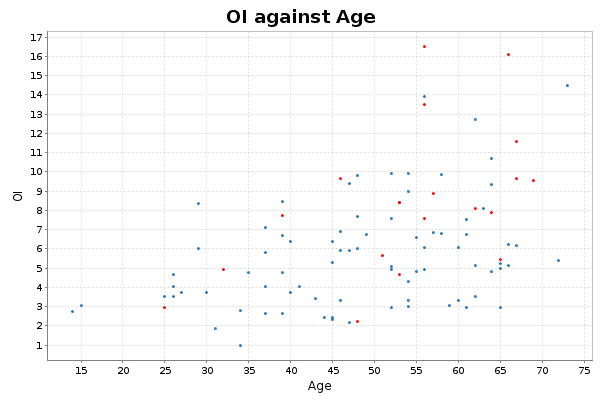
\includegraphics[width=\textwidth]{data}}
}

\frame{
\frametitle{Example: linear regression (6)}
\centerline{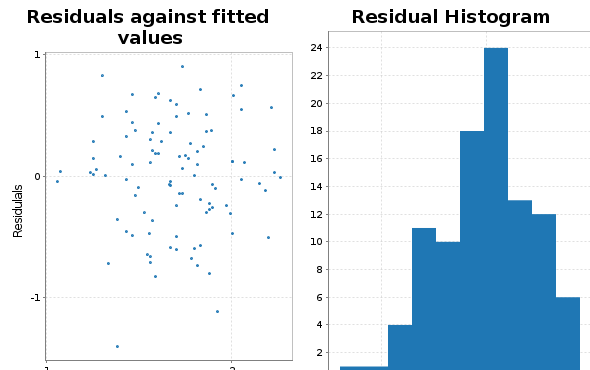
\includegraphics[width=0.8\textwidth]{resid}}
}


\begin{frame}[fragile]
\frametitle{Example: linear regression (7)}
{\scriptsize
\begin{lstlisting}[language=java]
scala> m.summary
res6: regression.LmSummary =
Residuals:
[5 x 1]
   Min -> -1.4005
    LQ -> -0.2918
Median ->  0.0308
    UQ ->  0.3211
   Max ->  0.8979
Coefficients:
[3 x 4]
                   OI     SE  t-val  p-val
               ------ ------ ------ ------
(Intercept) -> 0.8292 0.1777 4.6661 0.0000
        Age -> 0.0162 0.0035 4.6027 0.0000
    SexMale -> 0.3189 0.1157 2.7567 0.0070
Model statistics:
[6 x 1]
          RSS -> 20.0999
          RSE ->  0.4552
           df -> 97.0000
    R-squared ->  0.2621
Adjusted R-sq ->  0.2469
       F-stat -> 17.2265

scala> 
\end{lstlisting}
}
\end{frame}

\frame{
\frametitle{Example: linear regression (8)}
So we see that Scala could be just as convenient as R and similar languages for basic exploratory data analysis and visualisation, but this would require a little effort. If doing this again I would:
\begin{itemize}
\item Use \alert{Framian} rather than \alert{Saddle} as the basic data frame type
\item Use \alert{Wisp} for plotting and visualisation
\end{itemize}
It would then be useful to develop this into a library with functionality of the Python \alert{statsmodels} library
}


\begin{frame}[fragile]
\frametitle{Example: Gibbs sampler}
{\scriptsize
\begin{lstlisting}[language=java]
class State(val x: Double,val y: Double)
 
def nextIter(s: State): State = {
     val newX=rngG.nextDouble(3.0,(s.y)*(s.y)+4.0)
     new State(newX, 
          rngN.nextDouble(1.0/(newX+1),1.0/sqrt(2*newX+2)))
}
 
def nextThinnedIter(s: State,left: Int): State = {
   if (left==0) s 
   else nextThinnedIter(nextIter(s),left-1)
}
 
def genIters(s: State,current: Int,stop: Int,thin: Int): State = {
     if (!(current>stop)) {
        println(current+" "+s.x+" "+s.y)
        genIters(nextThinnedIter(s,thin),current+1,stop,thin)
     }
     else s
}
\end{lstlisting}
}
\end{frame}

\end{comment}

\subsection{Parallel particle filter}

\begin{frame}[fragile]
\frametitle{Example: Parallel particle filter}
{\scriptsize
\begin{lstlisting}[language=java]
(th: P) => {
  val x0 = simx0(n, t0, th).par
  @tailrec def pf(ll: LogLik, x: ParVector[S], t: Time, 
             deltas: List[Time], obs: List[O]): LogLik =
    obs match {
      case Nil => ll
      case head :: tail => {
        val xp = if (deltas.head == 0) x else 
               (x map { stepFun(_, t, deltas.head, th) })
        val w = xp map { dataLik(_, head, th) }
        val rows = sample(n, DenseVector(w.toArray)).par
        val xpp = rows map { xp(_) }
        pf(ll + math.log(mean(w)), xpp, t + deltas.head, 
                                        deltas.tail, tail)
      }
    }
  pf(0, x0, t0, deltas, obs)
}
\end{lstlisting}
}
\end{frame}

\begin{comment}

\frame{
\frametitle{Calling Scala from R (and vice versa)}
\begin{itemize}
\item R CRAN package \alert{jvmr} for bi-directional calling between R and Java and between R and Scala
\item Useful for calling out to computationally intensive routine written in Scala from an R session
\item Also useful for calling to R from Scala for a model-fitting procedure ``missing" from the Scala libraries
\item Can inline R code in Scala files and Scala code in R files
\end{itemize}
}

\end{comment}

\subsection{Spark}

\frame{
\frametitle{Spark}
\begin{itemize}
\item Spark is a scalable analytics library, including some ML (from Berkeley AMP Lab)
\item It is rapidly replacing Hadoop and MapReduce as the standard library for big data processing and analytics
\item It is written in Scala, but also has APIs for Java and Python (and experimental API for R)
\item Only the Scala API leads to both concise elegant code and good performance
\item Central to the approach is the notion of a \alert{resilient distributed dataset} (RDD) --- hooked up to Spark via a \alert{connector}
\end{itemize}
\alert{Lazy}, \alert{functional}, \alert{immutable} data workflows are what makes it all work --- that's why it's implemented in a language like Scala
}

\begin{frame}[fragile]
\frametitle{Spark example}
eg. maximising a logistic regression log-likelihood (gradient computation):
\begin{lstlisting}[language=java]
val gradient = points.map { p =>
  p.x * (1/(1+exp(-p.y*(w.dot(p.x))))-1) * p.y
}.reduce(_ + _)
\end{lstlisting}
Note that the RDD \texttt{points} could be terabytes big and distributed across a large cluster of nodes, yet the code is written as for any other immutable collection

The \alert{\texttt{map}} and \alert{\texttt{reduce}} operations naturally parallelise
\end{frame}


\subsection{Summary and further pointers}

\begin{comment}
\frame{
\frametitle{Summary}
\begin{itemize}
\item Strong arguments can be made that a language to be used as a platform for serious statistical computing should be general purpose, platform independent, \alert{functional}, statically typed and compiled
\item For basic exploratory data analysis, visualisation and model fitting, R works perfectly well (currently better than Scala)
\item Scala is worth considering if you are interested in any of the following:
  \begin{itemize}
  \item Writing your own statistical routines or algorithms
  \item Working with computationally intensive (parallel) algorithms
  \item Working with large and complex models for which an out-of-the-box solution doesn't exist in R
  \item Working with large data sets (big data)
  \item Integrating statistical analysis workflow with other system components (including web infrastructure, relational databases, no-sql databases, etc.)
  \end{itemize}
\end{itemize}
}
\end{comment}

\frame{
\frametitle{Summary}
\begin{itemize}
\item Strong arguments can be made that functional programming languages \alert{scale} better than conventional imperative languages
\item \alert{Concurrency} and \alert{parallelism} are difficult to manage in imperative languages due to \alert{shared mutable state}
\item Since functional languages avoid mutable state, writing concurrent and parallel code in functional languages is simple, natural and elegant
\item Learning a functional language will improve your programming, even if you return to an imperative language
\item Understanding the role of \alert{immutability} and \alert{referential transparency} in functional programming won't just make you a better programmer --- it will change how you think about \alert{computation} itself
\end{itemize}
}


\frame{
\frametitle{Links and further reading}
\begin{itemize}
\item Scala: \alert{\url{http://www.scala-lang.org/}} --- includes a comprehensive documentation section
\item Scala on wikipedia: \alert{\url{http://en.wikipedia.org/wiki/Scala_(programming_language)}}
\item My blog: \alert{\url{http://darrenjw.wordpress.com/}}
%\item A somewhat related talk with associated code examples: \alert{\url{https://github.com/darrenjw/statslang-scala}} (also merged into \alert{\url{https://github.com/csgillespie/statslang}})
\item Books:
  \begin{itemize}
  \item Programming in Scala (Odersky, Spoon, Venners)
  \item Functional programming in Scala (Chiusano and Bjarnason)
  \item Scala for machine learning (Nicolas)
  \item Several books on Spark just published or currently in press
  \end{itemize}
\item Coursera courses on \alert{FP in Scala} and \alert{Functional Reactive Programming}
\end{itemize}

}




\end{document}

